% Latex template for MA305 Project Report, Spring 2019
%%%%%%%%%%%%%%%%%%%%%%%%%%%%%%%%%%%%%%%%%%%%%%%%%%%%%%%%%%%
\documentclass[11pt]{article}
\usepackage{graphicx}
\usepackage[pdftex]{color}
\usepackage{multicol}
\newcommand{\cred} {\textcolor{red}}
\usepackage{fancyhdr}
\newcommand{\horrule}[1]{\rule{\linewidth}{#1}}      % Horizontal rule 
\usepackage{listings}
\definecolor{codegreen}{rgb}{0,0.6,0}
\definecolor{codegray}{rgb}{0.5,0.5,0.5}
\definecolor{codepurple}{rgb}{0.58,0,0.82}
\definecolor{backcolour}{rgb}{0.95,0.95,0.92}
\lstdefinestyle{mystyle}{
backgroundcolor=\color{backcolour},   
commentstyle=\color{codegreen},
keywordstyle=\color{magenta},
numberstyle=\tiny\color{codegray},
stringstyle=\color{codepurple},
basicstyle=\footnotesize,
breakatwhitespace=false,         
breaklines=true,                 
captionpos=b,                    
keepspaces=true,                 
numbers=left,                    
numbersep=5pt,                  
showspaces=false,                
showstringspaces=false,
showtabs=false,                  
tabsize=2
}
\lstset{style=mystyle}
\begin{document}
%%%%%%%%%% TITLE PAGE %%%%%%%%%%
\begin{center}
{\it MA448, Fall 2019  \hfill Embry-Riddle Aeronautical University
 }\\
\horrule{0.5pt} \\[0.4cm]
{\bf \Large  % change this
Project 1: Numerical Solution of ODEs
}\\
\horrule{2pt} \\[5cm]
%%%%%%%%%%%%%%%%%%%%
Brian Danaher, David Jefts, Jack Nguyen
\\[0.4cm]
\today % change this
\end{center}
\thispagestyle{empty}
\newpage
\begin{abstract}
\end{abstract}
\tableofcontents 
\newpage
%%%%%%%%%%  %%%%%%%%%%
\section{Introduction}\label{S:1}
%The text of this section.
It is a common occurrence in the natural sciences and engineering to encounter
differential equations which either cannot be solved analytically, or are too 
complex and time-consuming to attempt. For practical purposes, an approximation
of the solution is often sufficient to meet the demands of the problem, and a
multitude of algorithms and techniques have been developed to approximate 
ordinary differential equations (ODEs). This paper aims to evaluate these techniques by 
comparing them both to each other and to results published by professional mathematicians, 
and to educate the reader by solving a practical problem.
\section{Problem Statement}\label{S:2}
%The text of this section. 
\subsection{Part I}\label{S:2.1}
%
In this section, a multitude of different methods for solving ODEs are compared 
to one another by solving both a stiff and non-stiff equation. A stiff equation
is one in which the step size of the numerical methods used must be drastically
changed over the domain of the solution to maintain absolute stability. The 
methods evaluated in this way are the explicit implicit Euler's Method, the
implict Euler's Method, the Trapezoidal Method, the Classical Runge-Kutta 
fourth-order Method, the Fourth-order Adams-Bashforth-Moulton Method, and MATLAB's
builtin ODE solver ode45. These methods are evaluated by comparing the relative
errors of each solution relative to ode45 (a thoroughly tested algorithm), and 
the time required to solve each method.
\subsection{Part II}\label{S:2.2}
%
In the second part of this paper, a numerical method is developed for solving the
system of differential equations presented in the paper “Laura and Petrarch: An 
Intriguing Case of Cyclical Love Dynamics”. This paper aimed to develop a mathematical
model to simulate the emotional and inspirational cycle of the Italian poet Petrarch
and his love for Laura. The efficacy of the solver developed for this problem is
analysed by comparing the results to those in the paper.
\subsection{Part III}\label{S:2.3}
%
This paper concludes with simulating a pertinent real-world problem: that of the 
Lorenz problem, which arises in the study of dynamical systems. The Lorenz problem
is comprised of a series of three autonomous ODEs, and is noteworthy because of
the famous Lorentz attractor, which was discovered by analyzing this type of 
problem. The problem with (???) particular set of initial conditions and coefficients
is solved using the fourth-order Adams-Bashforth-Moulton Method.
\section{Methods}\label{S:3}
%Text introducing this section

The general form of a first-order ordinary differential equation is:
$$y'=f(t,y),\; y(t_0)=y_0$$
where the initial condition $y(t_0)=y_0$ provides a unique solution.

The explicit Euler's Method is perhaps the simplest and most straightforward of
the numerical methods used to solve ODEs, and was invented by Leonhard Euler who 
published it in his work Institutionum calculi integralis in 1768. Using a given
initial value $y_0$ at $t=t_0$ and number of steps $n$, the Explicit Euler's Method over
the domain $[t_0, t_f]$ is given by:
$$y_{n+1} = y_{n}+hf(t_{n}, y_{n}),\; h=\frac{t_f-t_0}{n}$$

The main advantage of this method is that it is simple to implement and that it
is self-starting. This method is a first-order approximation, and its error is
proportional to the step size: resulting in a relatively high error for a given
step size. The accuracy of Euler's Method can be increased by making the method 
implicit, where $y_n$ appears on both sides of the equation and must be algebraically
solved for. The implicit Euler's Method over the domain $[t_0, t_f]$ is given by:
$$y_{n+1} = y_{n}+hf(t_{n+1}, y_{n+1}),\; h=\frac{t_f-t_0}{n}$$

While this method is more accurate than the explicit Euler's Method, the computational
complexity is increased because a (possibly nonlinear) auxiliary equation must be
solved in order to isolate the right hand side. This must be done symbolically,
so either a computer algebra system or a person is needed to set the method up. In
this paper, the implicit equations were calculated by hand.

A similar method to the implicit Euler's Method is the Trapezoidal Method, which
is also an implicit (recursive) method. As the name suggests, this method uses the
equation of the area of a trapezoid to create the following implicit relation:
$$A_\mathrm{trapezoid}=\frac{h}{2}(b_{1}+b_{2})$$
$$y_{n+1}=y_{n}+\frac{h}{2}(f(t_{n}, y_{n})+f(t_{n+1}, y_{n+1})),\; h=\frac{t_f-t_0}{n}$$

Since this is also an implicit method, the term $y_{n+1}$ has to be isolated
using an auxiliary equation that can be solved either by hand or with a CAS.
In this paper, the auxiliary equation was calculated by hand.

Runge-Kutta Methods are a family of explicit numerical methods developed in the 18th
century by mathematicians Carl Runge and Wilhelm Kutta. These methods are given by:

$$y_{n+1}=y_{n}+h\sum_{i=1}^{s}b_{i}k_{i}$$
where
$$k_{1}=f(t_{n},y_{n})$$
$$k_{2}=f(t_{n}+C_{2}h,y_{n}+h(a_{2,1}k_{1}))$$
$$\vdots$$
$$k_{s}=f(t_{n}+C_{s}h,y_{n}+h(a_{s,1}k_{1}+a_{s,2}k_{2}+\dots+a_{s,s-1}k_{s-1}))$$

To specify a particular method, one needs both the number of stages $s$ and the
coefficients $a_{ij}$, $b_{ij}$, and $c_{ij}$. 
These coefficients are obtained by comparing the terms of the expression with the 
Taylor series expansion. The two
analysed in this paper are the classical fourth-order method, and the RK45 method.
These methods are both self-starting.
The classical fourth-order method is given by:

$$k_{1}=f(t_{n}, y_{n})$$
$$k_{2}=f\left(t_{n}+\frac{h}{2}, y_{n}+\frac{h}{2}k_{1}y_{n}\right)$$
$$k_{3}=f\left(t_{n}+\frac{h}{2}, y_{n}+\frac{h}{2}k_{2}y_{n}\right)$$
$$k_{4}=f(t_{n}+h, y_{n}+hk_{3}y_{n})$$
$$y_{n+1}=y_{n}+\frac{h}{6}(k{1}+2k_{2}+2k_{3}+k_{4})$$

As a fourth-order method, the error of this method is less than methods of a lesser
order. However, it is more computationally intensive than these methods. This
extra computational work can be mitigated if the method is adaptive, meaning it
changes its step size dynamically. The RK45 method is the most commonly used
adaptive RK4 method, in which the function is evaluated twice: once with a
fourth-order method, and once with a fifth-order method. Once both methods are 
evaluated in a given step, the difference between these two methods is used to
determine the step size for the next iteration. If the difference is less than some
user-specified range of tolerances, the step size for the next iteration is halved
to save on computational power. If the difference is greater than this range, the
step size for the next iteration is doubled to keep the approximation accurate.
This is most useful in stiff differential equations, where the value of $f(t,y)$
can vary significantly over a small interval.
One noteworthy use of this algorithm is in the MATLAB function ode45. The method
used in this algorithm is as follows:

$$k_{1}=f(t_{n}, y_{n})$$
$$k_{2}=f\left(t_{n}+\frac{h}{4}, y_{n}+\frac{1}{4}k_{1}\right)$$
$$k_{3}=f\left(t_{n}+\frac{3h}{8}, y_{n}+\frac{3}{32}k_{1}+\frac{9}{32}k_{2}\right)$$
$$k_{4}=f\left(t_{n}+\frac{12h}{13}, y_{n}+\frac{1932}{2197}k_{1}-\frac{7200}{2197}k_{2}+\frac{7296}{2197}k_{3}\right)$$
$$k_{5}=f\left(t_{n}+h, y_{n}+\frac{439}{216}k_{1}-8k_{2}+\frac{3680}{513}k_{3}-\frac{845}{4101}k_{4}\right)$$
$$k_{6}=f\left(t_{n}+\frac{h}{2}, y_{n}-\frac{8}{27}k_{1}+2k_{2}-\frac{3544}{2565}k_{3}+\frac{1859}{4101}k_{4}-\frac{11}{40}k_{5}\right)$$
$$y_{n+1}=y_{n}+h\left(\frac{25}{216}k_{1}+\frac{1408}{2565}k_{3}+\frac{2197}{4101}k_{4}-\frac{1}{5}k_{5}\right)$$
$$\tilde y_{n+1}=y_{n}+h\left(\frac{16}{135}k_{1}+\frac{6656}{12825}k_{3}+\frac{28561}{56430}k_{4}-\frac{9}{50}k_{5}+\frac{2}{55}k_{6}\right)$$

Where $y_{n+1}$ is the 4-th order approximation, and $\tilde y_{n+1}$ is the 5-th
order approximation. Note how $k_{2}$ is not used in either term. 

The last numerical method analysed in this paper is the 4-th order
Adams-Bashforth-Moulton Method. The family of Adams-Bashforth methods are modifications
of techniques used to approximate polynomials. These methods are rarely used by
themselves: the most common method used is the Adams-Bashforth-Moulton
predictor-corrector method. In this multistep method, a cursory
estimation of $y_{n+1}$ is calculated using the predictor, and is fine-tuned by
using the corrector. This method is given by:

$$p_{n+1}=y_{n}+\frac{h}{24}(-9f_{n-3}+37f_{n-2}-59f_{n-1}+55f_{n})$$
$$y_{n+1}=y_{n}+\frac{h}{24}(f_{n-2}-5f_{n-1}+19f_{n}+9f(t_{n+1}, p_{n+1}))$$

The main disadvantage of this method is that it is not self-starting. It requires 
4 values to start: $f_{n-3}$, $f_{n-2}$, $f_{n-1}$,and $f_{n}$. These four values 
can be calculated using any other numerical method. In this paper, both the 
explicit Euler's Method and classical RK4 Method were used to calculate these values.

\section{Solutions/Results}\label{S:4}
%Text introducing this section

\subsection{Part 1: Evaluation of ODE Solvers}
%

\subsubsection{Analysis of a nonstiff equation}
%

The nonstiff first-order ODE utilized in this section is given by:
$$y'=3+5\sin(t)+0.2y,\; y(0)=0$$

The domain of this problem was chosen to be $t\in [0,10]$ both to increase the 
magnitude of the differences betwen each method, and to capture the shape of
the solution. Since ode45 is the algorithm by which the other methods will be judged, 
the number of iterations of each method is the same as the number of steps chosen
by ode45 in this case: 65 steps. This consistent step size was also chosen to 
eliminate variability due to changing steps. The step size $h$ in this case is
0.1563, and the plot of the solutions given by each method are displayed in figure
1. The differences between each method over part of the domain are highlighted in figure 2.

\begin{figure} [ht]
\centering
        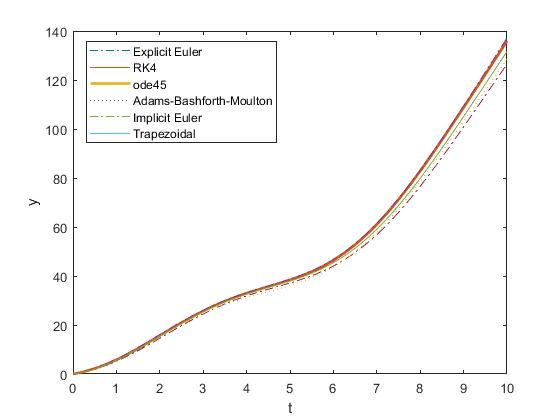
\includegraphics[totalheight=10cm]{Plot1aa.jpg}
    \caption{Solution of $y'=3+5sin(t)+0.2y, y(0)=0$ by various methods}
    \label{figure1}
\end{figure}

\newpage

\begin{figure} [ht]
\centering
        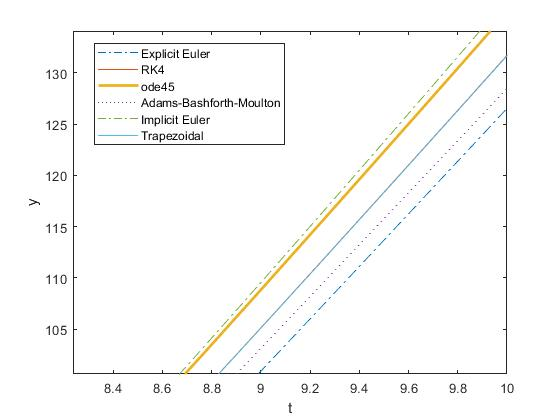
\includegraphics[totalheight=10cm]{Plot1ab.jpg}
    \caption{Detail of the solution curves}
    \label{figure2}
\end{figure}

A superficial examination of the solution curves reveals that the explicit Euler's
Method is closest to the solution provided by ode45, followed by the classical 
4-th order RK method, the trapezoidal method (which is so close to the RK4 method
as to have the curves overlap without zooming in considerably), the Adams-Bashforth-
Moulton Method, and the explicit Euler's Method. While the code written to execute
these algorithms also collects the time needed for each solver, these data are 
misleading if taken directly, because both of the implicit methods used (the implicit
Euler's Method and the Trapezoidal Method) required auxiliary equations that were
derived by hand, not by the MATLAB code. A brief derivation of each equation is
as follows:

Implicit Euler's Method:
$$y_{n+1}=y_{n}+hf(t_{n+1}, y_{n+1})$$
$$y_{n+1}=y_{n}+3h+5h\sin(t_{n+1})+0.2hy_{n+1}$$
$$y_{n+1}=\frac{y_{n}+3h+5h\sin(t_{n+1})}{(1-0.2h)}$$

Trapezoidal Method:
$$y_{n+1}=y_{n}+\frac{h}{2}(f(t_{n},y_{n})+f(t_{n+1},y_{n+1}))$$
$$y_{n+1}=y_{n}+\frac{3h}{2}+\frac{5h}{2}\sin(t_{n})+\frac{h}{10}y_{n}+\frac{3h}{2}+\frac{5h}{2}\sin(t_{n+1})+\frac{h}{10}y_{n+1}$$
$$y_{n+1}-\frac{h}{10}y_{n+1}=y_{n}+3h+\frac{5h}{2}\sin(t_{n})+\frac{h}{10}y_{n}+\frac{5h}{2}\sin(t_{n+1})$$
$$y_{n+1}(1-\frac{h}{10})=y_{n}+3h+\frac{5h}{2}\sin(t_{n})+\frac{h}{10}y_{n}+\frac{5h}{2}\sin(t_{n+1})$$
$$
y_{n+1}=\frac{y_{n}+3h+\frac{5h}{2}\sin(t_{n})+\frac{h}{10}y_{n}+\frac{5h}{2}\sin(t_{n+1})}{1-\frac{h}{10}}$$

In order to accurately represent the extra time MATLAB would need to derive these
equations for solving, the equations were derived using MATLAB's symbolic
toolbox, and the time for each derivation was collected. For reference, all MATLAB
code was executed on an Intel i5 7500 3.5 GHz CPU. The time needed to derive
the auxiliary equation for the Implicit Euler's Method is  0.1768 seconds,
and the auxiliary equation for the trapezoidal method took 0.1850 seconds to derive.
The time required for each solver is plotted against the final error compared to 
ode45's solution in Figure 3. The adjusted values (with the implicit methods 
augmented with the derivation time) are graphed in Figure 4.

\newpage

\begin{figure} [h]
\centering
        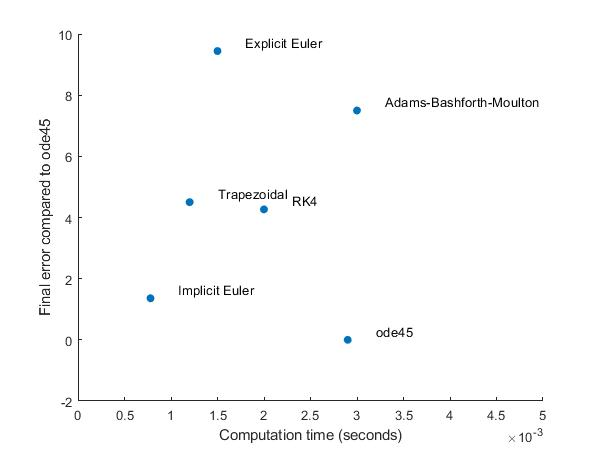
\includegraphics[totalheight=10cm]{scatter1.jpg}
    \caption{Computation time vs final error}
    \label{figure3}
\end{figure}

\begin{figure} [h]
\centering
        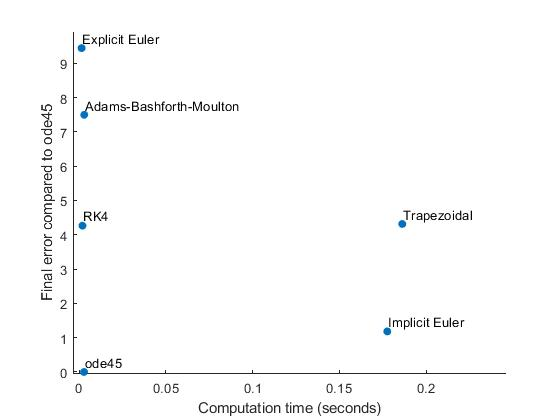
\includegraphics[totalheight=10cm]{scatter2.jpg}
    \caption{Computation and derivation time vs final error}
    \label{figure4}
\end{figure}

As demonstrated by these data, the implicit Euler's Method is is the method 
that has the lowest error per second of computation time when the equation
derivation is not factored in. However, both the implicit Euler's Method and 
the Trapezoidal rule take longer to compute than the explicit methods by two orders
of magnitude when the derivation time is accounted for: making these options
problematic choices if large numbers of equations have to be solved. When solving
non-stiff equations like this one, the best options are either ode45 or RK4: both
of which are Runge-Kutta methods. It will take further analysis on stiff equations
to determine which solver is the best overall, however.

\subsubsection{Analysis of a stiff equation}
%
The stiff nature of this problem necessitates a 
smaller domain than in the stiff problem. The equation in question is as follows: 
$$y'(t)=-1000y-e^{-t}, y(0)=0$$
Note how, during the beginning of the function, the slope of the solution is 
dominated by the term $-e^{-t}$ (which is approximately equal to one for small 
values of t), while it is later dominated by $-1000y$. This change in slope is so
drastic, that it causes the solvers to output nonsense answers with the same
number of steps (65) that was chosen in the previous
non-stiff analysis. The inconsistent nature of the solvers under these conditions
is illustrated in Figure 5. The only consistent solvers in this non-ideal scenario
are ode45, the trapezoidal method, and the RK4 method. The other methods either
diverge, or oscillate like the Adams-Bashforth-Moulton Method depending on the 
domain of the problem. An example of a solver diverging is illustrated in Figure
6 which shows a portion of the domain $t\in [0,1]$.

\begin{figure} [h]
\centering
        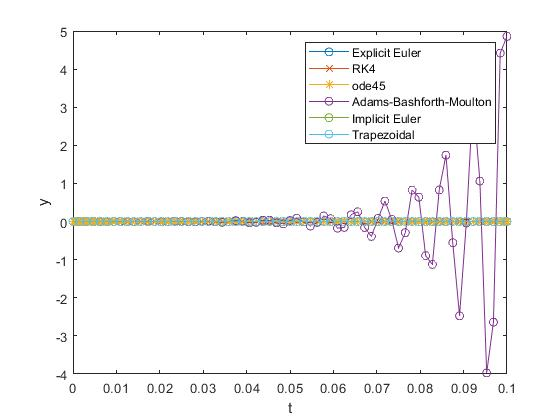
\includegraphics[totalheight=10cm]{figure3.jpg}
    \caption{An Oscillating Solution with an Improperly Large Domain}
    \label{figure5}
\end{figure}

\begin{figure} [h]
\centering
        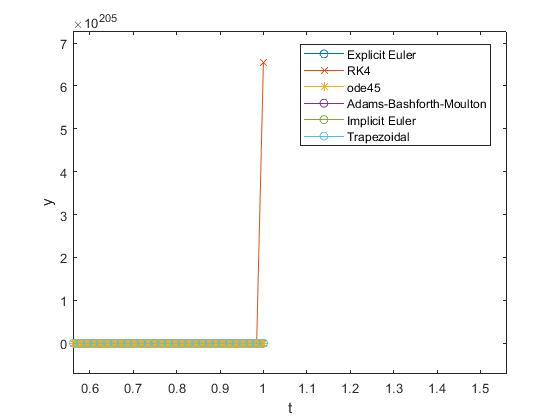
\includegraphics[totalheight=10cm]{divergence.jpg}
    \caption{A Divergent Solution with an Improperly Large Domain}
    \label{figure6}
\end{figure}

As ode45 is an adaptive algorithm which can change its step size dynamically,
this code chose 45 steps over $t\in [0,0.005]$ The number of steps for the other 
solvers were matched up with ode45 to maintain consistency, and the solution curves 
over $t\in [0,0.005]$ are plotted in Figure 7.

\begin{figure} [h]
\centering
        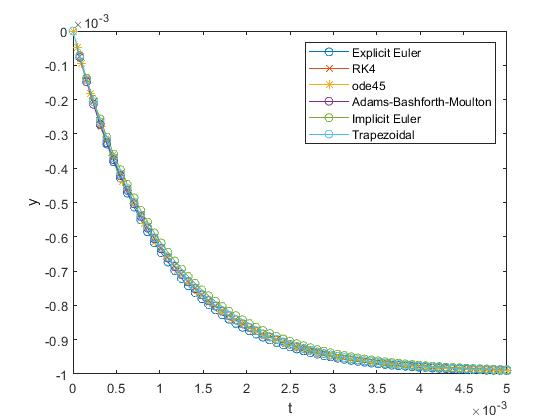
\includegraphics[totalheight=10cm]{figure4.jpg}
    \caption{Solution of $y'(t)=-1000y-e^{-t}, y(0)=0$}
    \label{figure7}
\end{figure}

The exponentially decaying curves of the solutions are such that they diverge
as the curves level out at around $t=0.0015$ seconds but converge very quickly afterwards.
For this reason, the error of each function when compared to ode45 is taken at the same
$t=0.0015$ seconds. In the same way as in the previous non-stiff analysis, the time each
solver took to complete was recorded, and the extra time MATLAB's symbolic
toolbox needed to find the equations of the implicit Euler and Trapezoidal methods
were added. In the symbolic toolbox, the implicit Euler's Method took 0.1926 seconds to solve,
and the Trapezoidal Method was solved in 0.2135 seconds. The derivations of these 
schemes by hand are as follows:
 
Implicit Euler's Method:
$$y_{n+1}=y_{n}+hf(t_{n+1}, y_{n+1})$$
$$y_{n+1}=y_{n}-1000hy_{n-1}-he^{-(t_{n+1})}$$
$$y_{n+1}=\frac{-he^{-t_{n+1}}}{1+1000h}$$

Trapezoidal Method:
$$y_{n+1}=y_{n}+\frac{h}{2}(f(t_{n},y_{n})+f(t_{n+1},y_{n+1}))$$
$$y_{n+1}=y_{n}-500hy_{n}-\frac{h}{2}e^{-t_{n}}-500hy_{n+1}-\frac{h}{2}e^{-t_{n+1}}$$
$$y_{n+1}(1+500h)=y_{n}-500hy_{n}-\frac{h}{2}(e^{-t_{n}}+e^{-t_{n+1}})$$
$$y_{n+1}=\frac{y_{n}-500hy_{n}-\frac{h}{2}(e^{-t_{n}}+e^{-t_{n+1}})}{1+500h}$$

The time required for each solver is plotted against the final error compared to 
ode45's solution in Figure 8. The adjusted values (with the implicit methods 
augmented with the derivation time) are graphed in Figure 9. The conclusions that
can be drawn about solver efficency are the same as in the nonstiff example. 
The implicit Euler's Method is is the method 
that has the lowest error per second of computation time when the equation
derivation is not factored in. However, both the implicit Euler's Method and 
the Trapezoidal rule take longer to compute than the explicit methods by two orders
of magnitude when the derivation time is accounted for: making these options
problematic choices if large numbers of equations have to be solved. When solving
non-stiff equations like this one, the best options are either ode45 or RK4: both
of which are Runge-Kutta methods.

\begin{figure} [h]
\centering
        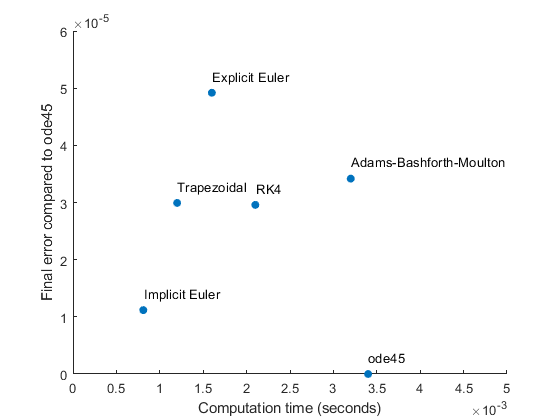
\includegraphics[totalheight=10cm]{error3.png}
    \caption{Computation and derivation time vs final error}
    \label{figure4}
\end{figure}

\begin{figure} [h]
\centering
        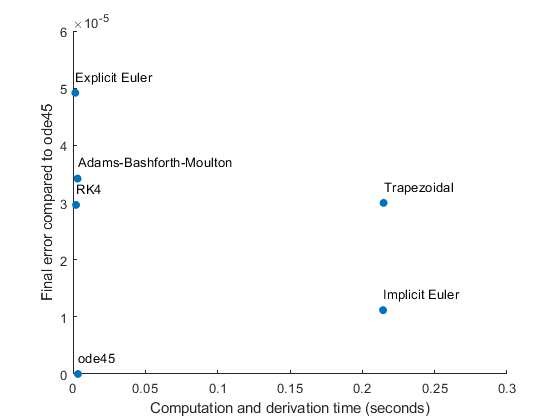
\includegraphics[totalheight=10cm]{error4.png}
    \caption{Computation and derivation time vs final error}
    \label{figure4}
\end{figure}

\subsection{Part 2: Cyclical Love Dynamics}
%
The system describing the emotional cycles of Petrarch and Laura were modeled by
mathematician Sergio Rinaldi is as follows:

$$\frac{dL}{dt}=-3.6L+1.2(P(1-P^{2})-1)$$
$$\frac{dP}{dt}=1.2P+6(L+\frac{2}{1+Z})$$
$$\frac{dZ}{dt}=-1.2Z+12P$$

Where L represents Laura's love for Petrarch, P represents Petrarch's love for
Laura, and Z represents Petrarch's level of poetic inspiration. Starting with the 
initial condition $L(0)=P(0)=Z(0)=0$, the system was solved using a scratch-programmed
RK45 method, and solved
over the interval
$t\in [0,21]$, where $t$ is measured in years. The solution curves plotted with time 
as the independent variable are graphed in figure 10, and the solutions in the
P-L and Z-P phase planes are plotted in figures 11 and 12, respectively. 

\begin{figure} [h]
\centering
        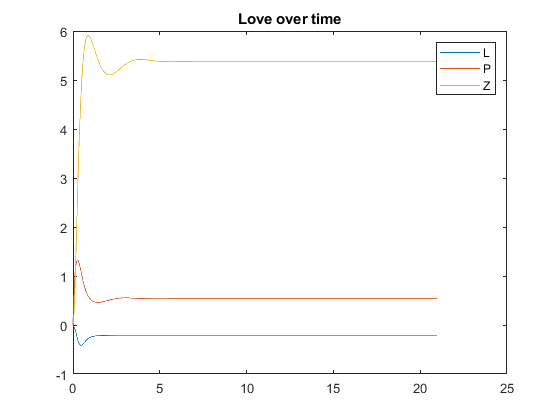
\includegraphics[totalheight=10cm]{love1.png}
    \caption{The emotional cycles of Laura and Petrach over 21 years}
    \label{figure5}
\end{figure}

\begin{figure} [h]
\centering
        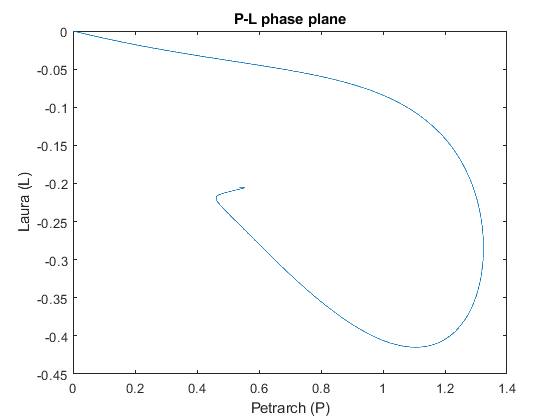
\includegraphics[totalheight=10cm]{love2.png}
    \caption{Petrarch's love for Laura (P) vs Laura's love for Petrarch (L)}
    \label{figure6}
\end{figure}

\begin{figure} [h]
\centering
        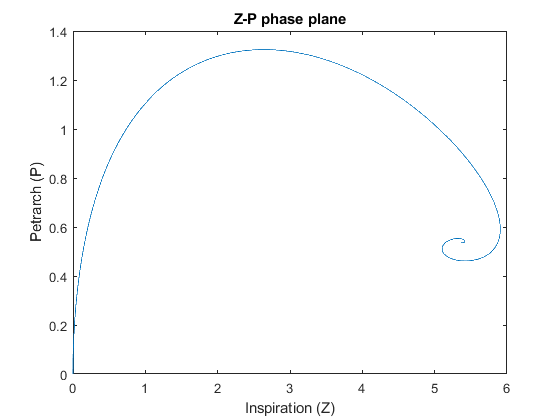
\includegraphics[totalheight=10cm]{love3.png}
    \caption{Petrarch's love for Laura (P) vs his inspiration level (Z)}
    \label{figure6}
\end{figure}

In order to validate these models, the coefficents within the system of differential
equations were changed to match the initial coefficents tested in Rinaldi's 
model:

$$\frac{dL}{dt}=-3L+1(P(1-P^{2})-1)$$
$$\frac{dP}{dt}=-P+5(L+\frac{2}{1+Z})$$
$$\frac{dZ}{dt}=-0.1Z+10P$$

A visual inspection of the plots given in the paper and the outputted solution 
curves confirms the accuracy of the RK45 method in this situation. The plots of
Rinaldi's solution  of L vs t and the RK45 solution are plotted in figures 13
and 14, respectivlely. The solution curves in the P-L and Z-P phase planes
solved by Rinaldi and the RK45 method are presented in in figues 15 and 16.

\begin{figure} [h]
\centering
        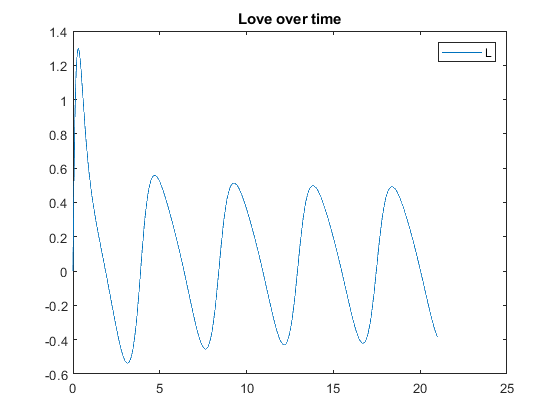
\includegraphics[totalheight=10cm]{evol1.png}
    \caption{The solution curve of Laura's love for Petrarch (L) vs time solved with RK45}
    \label{figure5}
\end{figure}

\begin{figure} [h]
\centering
        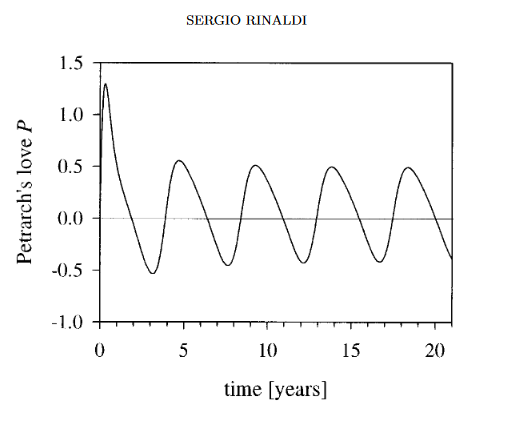
\includegraphics[totalheight=10cm]{sergio.png}
    \caption{The solution curve of Laura's love for Petrarch (L) vs time solved by Rinaldi}
    \label{figure6}
\end{figure}

\begin{figure} [h]
\centering
        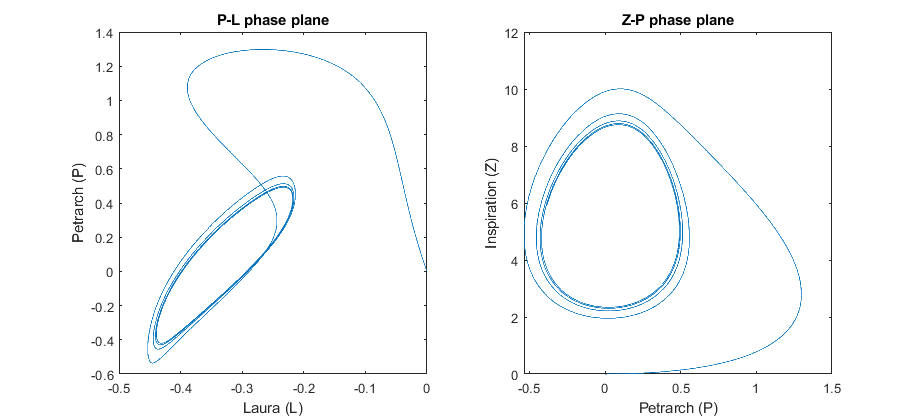
\includegraphics[totalheight=7cm]{evol2.png}
    \caption{The trajectories of the solutions in the L-P and P-Z phase planes provided by RK45}
    \label{figure6}
\end{figure}

\begin{figure} [h]
\centering
        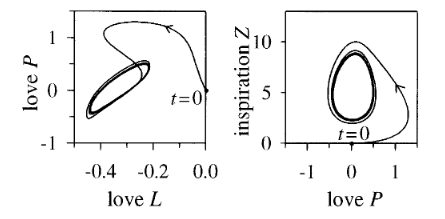
\includegraphics[totalheight=7cm]{pic1.png}
    \caption{The trajectories of the solutions in the L-P and P-Z phase planes provided by Rinaldi}
    \label{figure6}
\end{figure}

\subsection{Part 3: Solution of the Lorentz Problem}
%
The Lorentz problem analysed in this section is given by: 

$$\frac{dy_{1}}{dt}=10(y_{2}-y_{1})$$
$$\frac{dy_{2}}{dt}=y_{1}(28-y_{3})-y_{2}$$
$$\frac{dy_{3}}{dt}=y_{1}y_{2}-\frac{8}{3}y_{3}$$

This problem was solved using the fourth-order Adams-Bashforth-Moulton method in
Python with 2000 steps over the domain $t\in [0,20]$. This fine step size was chosen
because of the chaotic nature of the Lorentz problem, where even a small variance
in the solution can produce a drastic change in the curve at a later interval. 
When plotted with t as the independent variable, the solutions exhibit rapid 
oscillatory behavior as illustrated in figure 17. When plotted in the 
$y_{1}, y_{2}, y_{3}$ phase space, the solution takes the form of a Lorentz attractor:
a two-lobed twisting curve exhibited in figure 18.

\begin{figure} [h]
\centering
        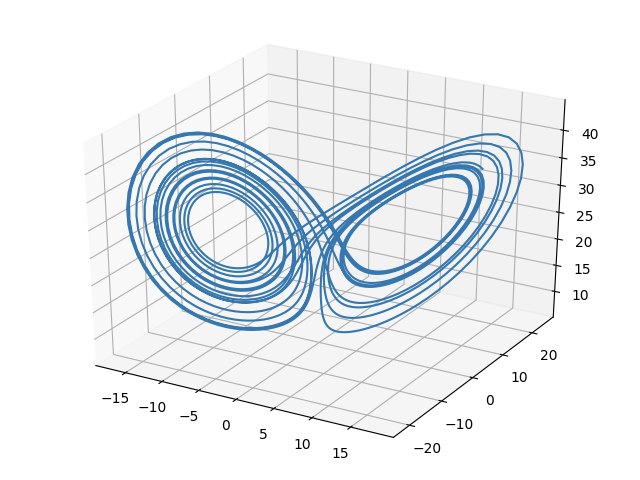
\includegraphics[totalheight=10cm]{figure8.png}
    \caption{The Lorentz Attractor For the System}
    \label{figure1}
\end{figure}

\newpage

\begin{figure} [h]
\centering
        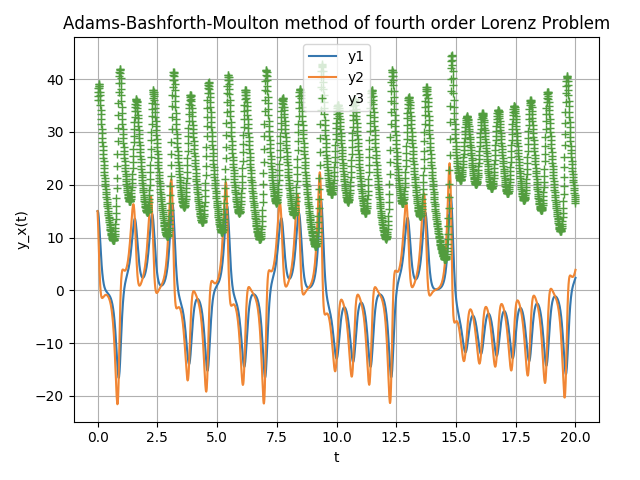
\includegraphics[totalheight=10cm]{original.png}
    \caption{The Solution Curves with Respect to Time}
    \label{figure2}
\end{figure}

\section{Discussion/Conclusions}\label{S:5}
%Text introducing this subsection

Interpret your solution physically, what we learn from it, comment on strengths and
weaknesses of the solution method, any nice features you want to brag about, 
possible ways to improve it (e.g. how to make it more accurate, more efficient), as
appropriate.
\begin{thebibliography}{100}
%List the materials used in the project. e.g., books, papers, web resources, codes, etc. 
\bibitem{a1}  
Heath, Michael T., Scientific Computing: An Introductory Survey, McGraw Hill, 2002.
%
%\bibitem{a2}
%
%\bibitem{a3} 
\end{thebibliography}
%\end{document}
%%%%%%%%%%%%%%%%%%%%%%%%%%%%%% section Appendix %%%%%%%%%%%%%%%%%%%%%
\newpage
\appendix 
\setcounter{section}{0}           
\section{Code}\label{S:A}
%
Code For Problem 1
\begin{lstlisting}[language=Matlab]
%Group 2, problem 1

clear;
clc;

%Initial Setup
y0 = 0;
t0 = 0;
n = 65;
tmax = 10;
h = (tmax-t0)/n;
explicit_euler = y0;
implicit_euler = y0;
trapezoidal = y0;
RK4 = y0;
AB4 = y0;
matlab = y0;
t = t0;
tmat = linspace(t, tmax, 65);

%Function definition
fy = @(t,y) 3+5*sin(t)+0.2*y;

tic
%Explicit Euler Method
for a=1:1:n-1
    explicit_euler = [explicit_euler, explicit_euler(1,a)+(h*fy(t, explicit_euler(1,a)))];
    t = t+h;
   
end
explicit_euler_time = toc;

%Implicit Euler Method
t = t0;

tic
for b=1:1:n-1
    t = t+h;
    implicit_euler = [implicit_euler, (implicit_euler(1,b)+3*h+5*h*sin(t))/(1-0.2*h)];
    
end
implicit_euler_time = toc;

%Trapezoidal Method
t = t0;

tic
for c=1:1:n-1
    t1 = t;
    t2 = t+h;
    
    trapezoidal = [trapezoidal, (trapezoidal(1,c)+3*h+(5*h/2)*sin(t1)+(h/10)*trapezoidal(1,c)+(5*h/2)*sin(t2))/(1-h/10)];
    t = t+h;
    
end
trapezoidal_time = toc;

%4th-order Classical RK Method
t = t0;

tic
for d=1:1:n-1   
    k1y = fy(t, RK4(1,d));
    k2y = fy(t+(h/2), RK4(1,d)+(k1y*(h/2)));
    k3y = fy(t+(h/2), RK4(1,d)+(k2y*(h/2)));
    k4y = fy(t+h, RK4(1,d)+k3y*h);
    
    RK4 = [RK4, RK4(1,d)+(h*(k1y+2*k2y+2*k3y+k4y)/6)];
    t = t+h;
    
end
RK4_time = toc;
    
%4th-order Adams Bashforth Method

%We will use the Explicit Euler Method calculated prior to start
abmat = [explicit_euler(1,1), explicit_euler(1,2), explicit_euler(1,3), explicit_euler(1,4)];
t = t0+(4*h);

tic
for e=4:1:n-1  
    ybar = abmat(1,e)+(h/24)*(55*fy(t, abmat(1,e))-59*fy(t-h, abmat(1,e-1))+37*fy(t-2*h, abmat(1,e-2))-9*fy(t-3*h, abmat(1,e-3)));
    fbar = fy(t+h, ybar);
    abmat = [abmat, abmat(1,e)+(h/24)*(9*fbar+19*fy(t, abmat(1,e))-5*fy(t-h, abmat(1,e-1))+fy(t-2*h, abmat(1,e-2)))];
    t=t+h;g
    
end
ABM_time = toc;

%ode45
tic
[ode45t, ode45y] = ode45(fy, [0,10], 0);
ode45_time = toc;

%Plot the data
plot(tmat, explicit_euler, '-o')
hold on
plot(tmat, RK4, '-x')
plot(ode45t, ode45y, '-*')
plot(tmat, abmat, '-o')
plot(tmat, implicit_euler, '-o')
plot(tmat, trapezoidal, '-o')

legend( 'Explicit Euler', 'RK4', 'ode45', 'Adams-Bashforth-Moulton', 'Implicit Euler', 'Trapezoidal')

\end{lstlisting} 

Code for Problem 2
\begin{lstlisting}[language=Matlab]
%% MA448 - Project: %%
%% #4 %%
%%%%%%%%%%%%%%%%%%%%%%
clear
clc
% differential equation:
f = @(t, y) [
(-3*y(1))+(1*(y(2)*(1-y(2)^2)-1));
(-y(2))+(5*(y(1)+(2/(1+y(3)))));
(-0.1*y(3))+(10*y(2))];
t0 = 0;
tmax = 21;
y0 = [0; 0; 0];
N = 100000;
t = linspace(t0, tmax, N+1);
% numerical solutions:
[Y, error] = RKF45(t0, tmax, y0, N, f);
% plot:
figure
plot(t, Y(:, 1), t, Y(:, 2), t, Y(:, 3))
legend('L', 'P', 'Z')
title('Love over time')
figure
plot(Y(:, 1), Y(:, 2))
title('P-L phase plane')




ylabel('Petrarch (P)')
xlabel('Laura (L)')


figure
plot(Y(:, 2), Y(:, 3))
title('Z-P phase plane')
ylabel('Inspiration (Z)')
xlabel('Petrarch (P)')
% RK45 method:
function [Y, error] = RKF45(t0, tmax, y0, N, f)
t = linspace(t0, tmax, N+1);
h = t(2) - t(1);
Y = [y0];
error = [zeros(size(y0))];
for i = 1:N
k1 = f(t(i), Y(:,i));
k2 = f(t(i) + h/4, Y(:,i) + h*k1/4);
k3 = f(t(i) + 3*h/8, Y(:,i) + 3*h*(k1+3*k2)/32);
k4 = f(t(i) + 12*h/13, Y(:,i) + h*(1932*k1-7200*k2+7296*k3)/2197);
k5 = f(t(i) + h, Y(:,i) + h*(439*k1/216-8*k2+3680*k3/513-845*k4/4104));
k6 = f(t(i) + h/2, Y(:,i) + h*(-8*k1/27+2*k2-3544*k3/2565+1859*k4/4104-11*k5/40));
Y(:,i+1) = Y(:,i) + h * (25*k1/216+1408*k3/2565+2197*k4/4104-k5/5);
error(:,i+1) = k1/360-128*k3/4275-2197*k4/75240+k5/50+2*k6/55;
end
Y = Y.';
end
\end{lstlisting} 

Code for problem 3
\begin{lstlisting}[language=Python]
import sys
import time

import numpy as np
import matplotlib.pyplot as plt
from scipy.integrate import odeint
from mpl_toolkits.mplot3d import Axes3D

"""
Write a code in Matlab/Python to implement the Adams-Bashforth-Moulton method of fourth order for the autonomous
system of ODEs.

Ỹn+1 = Yn + (h/24) * [55*F(Yn) − 59*F(Yn−1) + 37*F(Yn−2) − 9*F(Yn−3)]  -   Adams–Bashforth method
Yn+1 = Yn + (h/24) * 􏰆[9*F(Ỹn+1) + 19*F(Yn) − 5*F(Yn−1) + F(Yn−2)􏰇]      -   Adams–Moulton method

Use it to solve the following well known Lorenz problem that arises in the study of dynamical systems
dy1 = 10*(y2 - y1)          y1 is proportional to the rate of convection
dy2 = y1*(28 - y3) - y2     y2 is proportional to the horizontal temperature variation
dy3 = y1*y2 - (8/3)*y3      y3 is proportional to the vertical temperature variation
with initial conditions y1(0) = 15, y2(0) = 15, y3(0) = 36. Plot the solution curves for 0 ≤ t ≤ 20.
"""


def f(state, t):
    x, y, z = state  # unpack the state vector
    return sigma * (y - x), x * (rho - z) - y, x * y - beta * z  # derivatives


def rk4(rhs, y, t):
    M = len(y)
    N = len(t)
    Y = np.zeros((N, M))
    Y[0, :] = y
    dt = (t[-1] - t[0]) / N
    for n in range(N - 1):
        K1 = rhs(y, t[n])
        K2 = rhs(y + np.multiply(dt / 2, K1), t[n] + dt / 2)
        K3 = rhs(y + np.multiply(dt / 2, K2), t[n] + dt / 2)
        K4 = rhs(y + np.multiply(dt, K3), t[n] + dt)
        y = y + (np.multiply(dt / 6, K1) +
                 np.multiply(dt / 3, K2) +
                 np.multiply(dt / 3, K3) +
                 np.multiply(dt / 6, K4))
        Y[n + 1, :] = y
    return Y


def rk4_2(t, dt, y, N):
    state = [[y[0]], [y[1]], [y[2]]]
    for n in range(N - 1):
        # y1
        K1 = f(state, None)
        K2 = f([state[0][n] + 0.5 * dt * K1, state[1][n], state[2][n]])
        K3 = f([state[0][n] + 0.5 * dt * K2, state[1][n], state[2][n]])
        K4 = f([state[0][n] + dt * K3, state[1][n], state[2][n]])
        state[0].append(y[n] + dt * (K1 + 2 * K2 + 2 * K3 + K4) / 6)
        # y2
        K1 = f([state[0][n], state[1][n], state[2][n]])
        K2 = f([state[0][n], state[1][n] + 0.5 * dt * K1, state[2][n]])
        K3 = f([state[0][n], state[1][n] + 0.5 * dt * K2, state[2][n]])
        K4 = f([state[0][n], state[1][n] + dt * K3, state[2][n]])
        state[1].append(state[1][n] + dt * (K1 + 2 * K2 + 2 * K3 + K4) / 6)
        # y3
        K1 = f([state[0][n], state[1][n], state[2][n]])
        K2 = f([state[0][n], state[1][n], state[2][n] + 0.5 * dt * K1])
        K3 = f([state[0][n], state[1][n], state[2][n] + 0.5 * dt * K2])
        K4 = f([state[0][n], state[1][n], state[2][n] + dt * K3])
        state[2].append(state[2][n] + dt * (K1 + 2 * K2 + 2 * K3 + K4) / 6)
    return state


# lorenz parameters
rho = 28
sigma = 10.0
beta = 8.0 / 3.0

""" START OF MAIN """
t0 = 0
tmax = 20
N = 2001
t, h = np.linspace(t0, tmax, N, retstep = True)
# print('T:', list(t))

state0 = [15, 15, 36]

""" get the first 3 spots in each function """
states = rk4(f, state0, t[0:4])

y1 = states[0]
y2 = states[1]
y3 = states[2]
print("Initial + 3 Orders:", states[0:4], sep = '\n', end = '\n\n')
time.sleep(0.1)

for n in range(3, N):
    state = states[n]
    # print(state)
    # calculate Ÿ values
    # Ỹn+1 = Yn + (h/24) * [55*F(Yn) − 59*F(Yn−1) + 37*F(Yn−2) − 9*F(Yn−3)]
    y_tilde = state + (h / 24) * (np.multiply(55, f(state, t[n]))
                                  - np.multiply(59, f(states[n - 1], t[n]))
                                  + np.multiply(37, f(states[n - 2], t[n]))
                                  - np.multiply(9, f(states[n - 3], t[n])))
    # calculate next Y value
    # Yn+1 = Yn + (h/24) * 􏰆[9*F(Ỹn+1) + 19*F(Yn) − 5*F(Yn−1) + F(Yn−2)􏰇]
    state1 = states[n] + (h / 24) * (np.multiply(9, f(y_tilde, t[n]))
                                     + np.multiply(19, f(state, t[n]))
                                     - np.multiply(5, f(states[n - 1], t[n]))
                                     + np.multiply(1, f(states[n - 2], t[n])))
    states = np.vstack((states, state1))

""" plot everything """
y1 = []
y2 = []
y3 = []
print("=========================================================================")
print("    n\t y1\t\t\t\t\ty2\t\t\t\t\t y3", end = '\n')
for n in range(N):
    y_1 = states[n][0]
    y1.append(y_1)
    y_2 = states[n][1]
    y2.append(y_2)
    y_3 = states[n][2]
    y3.append(y_3)
    print(' {:4d}\t{:0.15f}\t{:0.15f}\t{:0.15f}'.format(n, y_1, y_2, y_3))
print("=========================================================================")

plt.plot(t, y1, '-', t, y2, '-', t, y3, '+')
plt.title("Adams-Bashforth-Moulton method of fourth order Lorenz Problem")
plt.legend(['y1', 'y2', 'y3'], loc = 'best')
plt.ylabel('y_x(t)')
plt.xlabel('t')
plt.grid()
plt.show()

time.sleep(0.1)

# 3D representation
title = 'Lorenz System - $\\rho ={:.4g}, \\sigma ={:.4g}, \\beta ={:.4g}$'.format(rho, sigma, beta)
fig = plt.figure()
ax = fig.gca(projection = '3d')
# fig.set_title(title)
ax.plot(y1, y2, y3)
ax.set_title(title)
plt.show()

\end{lstlisting} 


\end{document}